\documentclass[12pt,a4paper,parskip=full]{scrartcl}

\usepackage{bbding}
\usepackage[utf8]{inputenc}
\usepackage{pifont}
\usepackage{wasysym}
\usepackage[margin=1in]{geometry}
\geometry{letterpaper}
\usepackage{xcolor}
\definecolor{red}{HTML}{cc0000}
\definecolor{gray}{HTML}{666666}
\usepackage{sectsty}
\sectionfont{\color{red}}
\subsectionfont{\color{red}}
\usepackage{graphicx}
\usepackage{hyperref}
\usepackage{amssymb}
\usepackage[style=footnote-dw]{biblatex}
\bibliography{S@SGuideBib}
\setlength\bibitemsep{0.5\baselineskip}

\usepackage{enumitem}
\setitemize{noitemsep}
% \setlist{noitemsep, topsep=-5pt}
% \setlength\itemsep{-0.10em}

\renewcommand{\labelitemi}{$\cdot$}
\renewcommand{\labelitemii}{$\cdot$}
\makeatletter
\let\latexl@section\l@section
\def\l@section#1#2{\begingroup\let\numberline\@gobble\latexl@section{#1}{#2}\endgroup}
\makeatother

\usepackage[T1]{fontenc}
\fontfamily{verdana}

\usepackage{scrlayer-scrpage}{}
\makeatletter
\renewcommand{\@seccntformat}[1]{}
\makeatother

\setlength\parindent{0pt}{}

\title{\Huge{\color{red}\textbf{Der Scrum@Scale
\textsuperscript{\copyright}
Guide}}}
\subtitle{\color{gray}Der gültige Leitfaden für Scrum@Scale:\\ Skalierung, die funktioniert}
% \author{}
\date{}


\begin{document}

%\tableofcontents
%\newpage

\section{Zweck des Scrum@Scale Guides}
Scrum, wie ursprünglich im Scrum Guide beschrieben, ist ein Rahmenwerk,
um komplexe Produkte mit Hilfe eines einzelnen Teams zu entwickeln,
auszuliefern und zu erhalten. Seit seiner Einführung hat sich die Anwendung
auf die Erstellung von Produkten, Prozessen, Services und Systemen erweitert,
die der Zusammenarbeit mehrerer Teams bedürfen. Scrum@Scale wurde entwickelt,
um dieses Ökosystem von Teams effektiv zu koordinieren, so dass es die gesamte
Strategie der Organisation optimiert. Es erreicht dieses Ziel, indem es mit
einer skalierungsfreien Architektur eine "minimal überlebensnotwendige
Bürokratie" aufbaut. Diese weitet die Arbeitsweise eines einzelnen Scrum Teams
organisch auf die Organisation aus.

Dieser Leitfaden enthält die Definitionen der Komponenten, aus denen das
Scrum@Scale Rahmenwerk besteht, einschließlich seiner skalierten Rollen,
skalierten Events, Unternehmensartefakte, sowie den Regeln, die diese
zusammenhalten.

Dr. Jeff Sutherland entwickelte Scrum@Scale auf Basis der fundamentalen
Prinzipien hinter Scrum, der Complex Adaptive Systems Theorie, Spieltheorie und
objektorientierter Technologie. Dieser Guide wurde mit Hilfe des Inputs vieler
erfahrener Scrum Anwender auf Basis ihrer Praxiserfahrungen entwickelt. Ziel
dieses Guides ist, dass Leser Scrum@Scale selbstständig implementieren können.

\subsection{Warum Scrum@Scale?}
Scrum wurde dafür entwickelt, ein einzelnes Team dazu zu befähigen, in
nachhaltiger Geschwindigkeit mit seiner optimalen Leistungsfähigkeit zu
arbeiten. In der Anwendung hat sich ergeben, dass mit zunehmender Anzahl der
Scrum Teams in der Organisation der Output (funktionierendes Produkt) und die
Velocity sanken (aufgrund von Abhängigkeiten zwischen Teams und Doppelarbeiten).
Es wurde deutlich, dass ein Rahmenwerk zur effektiven Koordination dieser Teams
benötigt wurde, um lineare Skalierbarkeit zu erreichen. Scrum@Scale ist designt,
um dieses Ziel mit Hilfe seiner skalierungsfreien Architektur zu erreichen.


Bei der Verwendung einer skalierungsfreien Architektur ist die Organisation
nicht darauf beschränkt, sich in eine Richtung zu entwickeln, die durch eine
Reihe von zufälligen Regeln bestimmt wird; stattdessen kann sie organisch nach
ihren eigenen Bedürfnissen und mit nachhaltiger Veränderungsgeschwindigkeit
wachsen, was den Gruppen von Individuen, die die Organisation ausmachen,
entgegenkommt. Die Einfachheit des Scrum@Scale-Modells ist essenziell für eine
skalierungsfreie Architektur. Diese Einfachheit vermeidet die Einführung von
zusätzlicher Komplexität, die die Teamproduktivität senkt, wenn weitere Teams
entstehen.

Scrum@Scale ist designt, durch die Organisation als Ganzes zu skalieren: durch
alle Abteilungen, Produkte und Services. Es kann über mehrere Domänen hinweg
und in allen Arten von Organisationen in Industrie, Verwaltung und Lehre
angewendet werden.

\subsection{Definition von Scrum@Scale}
Scrum(n): Ein Rahmenwerk, innerhalb dessen Menschen komplexe adaptive
Aufgabenstellungen angehen können, und durch das sie in die Lage versetzt
werden, produktiv und kreativ Produkte mit höchstmöglichem Wert auszuliefern.

Der Scrum Guide ist das minimale Feature Set. Es ermöglicht Inspektion und
Anpassungsfähigkeit durch radikale Transparenz, um Innovation,
Kundenzufriedenheit, Leistungsfähigkeit und Teamzufriedenheit zu steigern.

Scrum@Scale: Ein Rahmenwerk, innerhalb dessen Netzwerke von Scrum Teams, die
konsequent nach dem Scrum Guide arbeiten, komplexe adaptive Aufgabenstellungen
angehen können, und durch das sie in die Lage versetzt werden, produktiv und
kreativ Produkte mit höchstmöglichem Wert auszuliefern.

\textbf{ANMERKUNG:} Diese ``Produkte'' können Hardware, Software, komplexe
integrierte Systeme, Prozesse, Services etc. sein, abhängig von der Domäne,
in der die Scrum Teams arbeiten.

Scrum@Scale ist:
\begin{itemize}
\item Leichtgewichtig – die minimal überlebensnotwendige Bürokratie
\item Einfach zu verstehen – besteht ausschließlich aus Scrum Teams
\item Schwierig zu meistern – benötigt die Implementierung eines neuen Betriebsmodells
\end{itemize}


Scrum@Scale ist ein Rahmenwerk für die Skalierung von Scrum. Es vereinfacht Skalierung radikal, indem es Scrum für die Skalierung von Scrum einsetzt.

In Scrum wird die Verantwortung über das ``Was'' von der Verantwortung über das
``Wie'' getrennt. Genauso verhält es sich bei Scrum@Scale, damit
Verantwortlichkeit und Zuständigkeit explizit vereinbart werden. Ziel ist es,
unnötige organisatorische Konflikte zu vermeiden, die Teams davon abhalten,
ihre optimale Produktivität zu erreichen.

Scrum@Scale besteht aus Komponenten, die es einer Organisation erlauben, ihre
Transformationsstrategie und Umsetzung auf ihre Bedürfnisse anzupassen. Sie gibt
ihnen die Möglichkeit, die Transformation auf Bereiche zu konzentrieren, in
denen Veränderung am wertvollsten oder am nötigsten ist, um sich anschließend
weiteren Bereichen zuzuwenden.

Durch die Trennung der Zuständigkeiten enthält Scrum@Scale zwei Zyklen: den
Scrum Master Zyklus (das ``Wie'') und den Product Owner Zyklus (das ``Was'').
Jeder dieser beiden berührt den anderen an zwei Stellen. Zusammengenommen
erschaffen diese Zyklen ein mächtiges Rahmenwerk, um den Einsatz mehrerer Teams
entlang eines gemeinsamen Pfades zu koordinieren.

\subsection{Die Komponenten des Scrum@Scale\textregistered ~Rahmenwerkes}

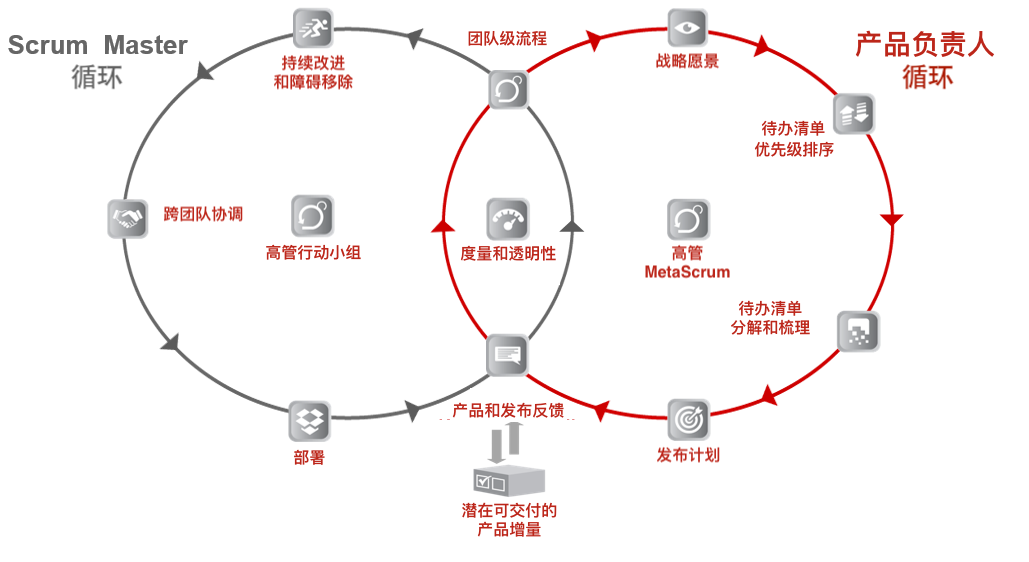
\includegraphics[width=1.0\linewidth]{SMPO-Cycle.png}

\subsection{Wertebasierte Kultur}
Neben der Trennung der Verantwortung über das ``Was'' und das ``Wie'', zielt
Scrum@Scale darauf ab, gesunde Organisationen mit einer Kultur zu schaffen, die
wertebasiert und empirisch arbeitet. Die Scrum Werte sind:
Offenheit, Mut, Fokus, Respekt und Selbstverpflichtung. Diese Werte fördern
empirische Entscheidungsfindung, die auf den drei Säulen
Transparenz, Inspektion und Adaption ruht.

Offenheit bringt Transparenz in alle Tätigkeiten und Prozesse. Ohne Transparenz
gibt es keine Möglichkeit, diese aufrichtig zu überprüfen (Inspektion) und zu
versuchen, sie zu verbessern (Adaption). Es bedarf Mut, um beherzte Sprünge zu
tun, die nötig sind, um Wert schneller innovativ zu liefern.

Fokus und Selbstverpflichtung beziehen sich darauf, wie wir unseren
Arbeitsverpflichtungen nachkommen und setzen die Lieferung von Wert an den
Kunden an erste Stelle. Letztendlich muss alles dies in einer Umgebung
geschehen, die auf Respekt für die Individuen basiert, ohne die nichts
geschaffen werden kann.

Scrum@Scale hilft Organisationen dabei, zu gedeihen, indem es ein
transformationales Führungsmodell unterstützt. Dies fördert ein positives
Umfeld für nachhaltige Arbeitsgeschwindigkeit und unsere Verpflichtung,
Kundenwert in den Fokus unserer Bemühungen zu setzen.

\subsection{Mit Scrum@Scale starten}
Um große Netzwerke von Teams aufzubauen, ist es entscheidend, zuerst ein
skalierbares \textbf{Referenzmodell} mit einem kleinen Set von Teams zu
entwickeln. Jegliche Defizite der Scrum-Einführung summieren sich auf, sobald
mehrere Teams eingesetzt werden. Viele der anfänglichen Skalierungs-
schwierigkeiten werden organisatorische Richtlinien und Vorgehensweisen oder
Entwicklungspraktiken sein, die die Teams blockieren und frustrieren.

Deswegen besteht die erste Herausforderung darin, ein kleines Set von Teams
zu kreieren, die gutes Scrum implementieren. Das wird am besten durch die
Schaffung eines \textbf{Executive Action Team (EAT)} erreicht, das für die
Entwicklung und Ausführung der Transformationsstrategie verantwortlich ist.
Das EAT muss aus Personen bestehen, die politisch und finanziell ermächtigt
sind, die Existenz des Referenzmodells zu gewährleisten. Dieses Set von Teams
arbeitet organisatorische Hindernisse ab, die Agilität blockieren. Es setzt
ein arbeitsfähiges Referenzmodell für die Organisation um, das als Muster
 verwendet werden, um Scrum unternehmensweit zu skalieren.

Sobald das Referenzmodell von Teams schneller wird, werden Hindernisse und
Flaschenhälse sichtbar, die Auslieferung verzögern, Verschwendung produzieren
oder die Business Agility der Organisation behindern. Der effektivste Weg, um
diese Probleme zu beseitigen, ist Scrum über die gesamte Organisation
auszubreiten, so dass der gesamte Wertstrom optimiert wird.

Scrum@Scale schafft lineare Skalierbarkeit der Produktivität durch die
Sättigung der Organisation mit Scrum und die organische Verteilung von Velocity
und Qualität, konsistent mit der unternehmensspezifischen Strategie, den
Produkten und Services.

\section{Scrum Master Zyklus}
\subsection{Team Level Prozess}
Der \textbf{Team Level Prozess} cDer Team-Level Prozess stellt den ersten Berührungspunkt
zwischen Scrum Master und Product Owner Zyklus dar und ist klar im Scrum Guide beschrieben.
Er ist besteht aus drei Artefakten, fünf Events und drei Rollen.
Die Ziele des Team Level Prozesses sind:
\begin{itemize}
\item den Fluss an fertiger und qualitätsgeprüfter Arbeit zu maximieren
\item die Leistungsfähigkeit des Teams mit der Zeit zu erhöhen.
\item so zu arbeiten, dass es nachhaltig und bereichernd für das Team ist.
\item ie Feedbackschleife zum Kunden zu beschleunigen.
\end{itemize}

\subsection{Das ``Wie'' koordinieren – Das Scrum of Scrums}
Ein Set von Teams, das sich koordinieren muss um Wert an einen Kunden zu liefern, bildet ein \textbf{``„Scrum of Scrums'' (SoS)}. Dieses Team ist selbst ein Scrum Team. Es ist für ein vollständig integriertes Set von potenziell auslieferfähigen Inkrementen am Ende jedes Sprints von allen teilnehmenden Teams verantwortlich. Ein SoS funktioniert als ein Releaseteam, und muss in der Lage sein, seinen Kunden direkt Wert zu liefern. Um das effektiv leisten zu können, muss es konsistent mit dem Scrum Guide sein, also seine eigenen Rollen, Artefakte und Events haben:

Rollen:

Das SoS braucht alle Fähigkeiten, die notwendig sind, um ein vollständig integriertes, potenziell auslieferbares Inkrement am Ende jedes Sprints zu liefern. (Es könnte erfahrene Architekten, Führungspersonen aus der Qualitätssicherung, Mitglieder des Product Owner Teams und andere operativen Fähigkeiten benötigen.) Der Scrum Master des Scrum of Scrums heißt \textbf{Scrum of Scrums Master (SoSM)}.

Events:

Der SoSM sollte ein Backlog Refinement Event ermöglichen, in dem entschieden wird, welche Hindernisse ``ready'' sind, um beseitigt zu werden, wie sie am besten gelöst werden können und woran das Team erkennt, dass etwas ``done'' ist. Diese Product Backlog Einträge / Artefakte zur Beseitigung von Hindernissen werden für die Teams im gleichen und einzigen Backlog priorisiert, das durch das MetaScrum erstellt wird.
Besondere Aufmerksamkeit sollte die SoS Retrospektive erhalten, in der die Teamvertreter alle Lernerfahrungen oder Prozessverbesserungen teilen, mit denen ein individuelles Team Erfolg hatte, um diese bestmöglichen Praktiken innerhalb der Teams des SoS zu teilen.
Da das SoS in Echtzeit auf die von den beteiligten Teams gemeldeten Hindernisse reagieren können muss, muss mindestens ein Teamvertreter (normalerweise der Team Scrum Master) von jedem teilnehmenden Team an einem \textbf{Scaled Daily Scrum (SDS)} teilnehmen. Das SDS Event spiegelt das Daily Scrum insofern, dass es die Zusammenarbeit und Leistungsfähigkeit des Netzwerkes von Teams optimiert. Je nach Bedarf kann jede Person und jegliche Anzahl von Personen teilnehmen.

Zusätzlich ist das SDS:

\begin{itemize}
\item time-boxed auf 15 Minuten oder weniger
\item von einem Vertreter jedes Teams, inklusive des Product Owner Teams, besucht
\item ein Forum, in dem die Vertreter besprechen was gut läuft, was fertiggestellt wird und wie die Teams effektiver zusammenarbeiten können. Beispielsweise kann besprochen werden:
\begin{itemize}
\item Welche Hindernisse hat mein Team, die es davon abhalten, das Sprintziel zu erreichen (oder die das kommende Release beeinflussen)?
\item Tut mein Team irgendetwas, das ein anderes Team davon abhält, sein Sprintziel zu erreichen (oder was das kommende Release beeinflusst)?
\item Haben wir neue Abhängigkeiten zwischen Teams entdeckt, oder bekannte Abhängigkeiten auflösen können?
\item Welche Verbesserungen haben wir entdeckt, die teamübergreifend genutzt werden können?
\end{itemize}
\end{itemize}

\subsection{Der Scrum of Scrums Master (SoSM)}
Der Scrum of Scrums Scrum Master (SoSM) ist für die Auslieferung der gemeinsamen Teamleistungen verantwortlich und muss:
\begin{itemize}
\item Fortschritt sichtbar machen
\item ein Impediment Backlog für die Organisation sichtbar machen.
\item Hindernisse beseitigen, die die Teams nicht selbst beseitigen können.
\item Die Priorisierung von Hindernissen mit besonderer Aufmerksamkeit auf Abhängigkeiten zwischen Teams und die Verteilung von Product Backlog Einträgen ermöglichen
\item die Effektivität des Scrum of Scrums verbessern.
\item eng mit den Product Ownern zusammenarbeiten, um ein potenziell auslieferbares Produktinkrement mindestens am Ende jedes Sprints bereitzustellen.
\item die Lieferungen der Teams mit den Releaseplänen des Product Owners koordinieren.
\end{itemize}

\subsection{Das SoS skalieren}
Abhängig von der Größe der Organisation oder Implementierung, kann mehr als ein
SoS benötigt werden, um ein sehr komplexes Produkt liefern zu können. In diesen
Fällen kann ein textbf\{Scrum of Scrum of Scrums (SoSoS)} aus mehreren Scrum of Scrums
gebildet werden. Das SoSoS ist ein organisches Muster von Scrum Teams, das
unendlich skalierbar ist. Jedes SoSoS sollte SoSoSMaster und skalierte Versionen
jedes Artefakts \& Events haben.

Die Skalierung des SoS reduziert die Anzahl der Kommunikationswege innerhalb
der Organisation, so dass Komplexität gekapselt ist. Das SoSoS verbindet sich
mit dem SoS genauso, wie ein SoS sich mit einem einzelnen Team verbindet. Das
ermöglicht lineare Skalierbarkeit.

\pagebreak
Beispieldiagramme:

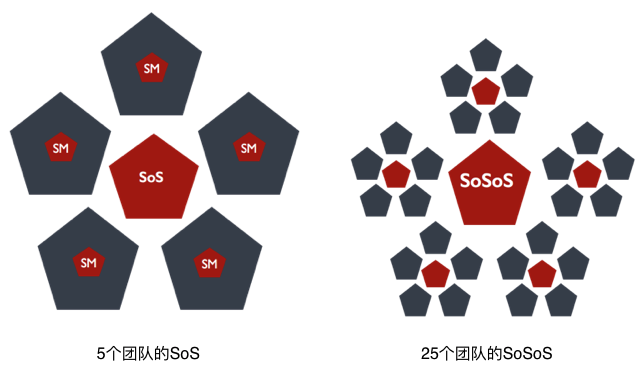
\includegraphics[width=1.0\linewidth]{Sos-R2.png}

\textbf{\textsc{Anmerkung:}} Während der Scrum Guide die optimale Teamgröße als
drei bis neun Personen definiert, haben Harvard-Untersuchungen festgestellt,
dass die optimale Teamgröße 4.6 Personen beträgt. (Fußnote 1). Experimente mit
hochperformanten Scrum Teams haben wiederholt gezeigt, dass vier oder fünf
Personen die optimale Größe ist. Für eine lineare Skalierbarkeit ist es
wesentlich, dass dieses Muster für die Gesamtzahl von Teams in einem SoS
beibehalten wird. Deswegen wurden in diesem wie in den folgenden Diagrammen
Fünfecke ausgewählt, um ein fünfköpfiges Team darzustellen. Diese Diagramme
sollen nur als Beispiele dienen, Ihr eigenes Organisationsdiagramm kann stark
hiervon abweichen.

\subsection{Das Executive Action Team}
Das Scrum of Scrums für die gesamte agile Organisation ist das
\textbf{Executive Action Team (EAT)}. Dieses Führungsteam kreiert eine agile
Blase in der Organisation, in der das Referenzmodell mit seinen eigenen
Richtlinien und Vorgehensweisen arbeitet. Diese Blase schließt sich effektiv
an alle Teile der Organisation an, die nicht agil sind. Dem EAT gehört das
agile Ökosystem, es implementiert die Scrum Werte und stellt sicher, dass die
Scrum Rollen geschaffen und unterstützt werden.

Das EAT ist die letzte Station für Hindernisse, die von dem SoSs gemeldet und
nicht von ihnen selbst beseitigt werden können. Daher muss das EAT aus Personen
bestehen, die politisch und finanziell bevollmächtigt sind, diese Hindernisse
zu beseitigen. Das EAT koordiniert mehrere SoSs (oder SoSoSs) und sorgt für die
Anschlüsse an die nicht-agile Organisationsteile. Wie jedes Scrum Team benötigt
das EAT einen Product Owner und einen Scrum Master und trifft sich täglich.
Genauso muss es ein transparentes Backlog haben


%\pagebreak
Beispieldiagramm zeigt ein EAT, das 5 Gruppierungen mit 25 Teams koordiniert:

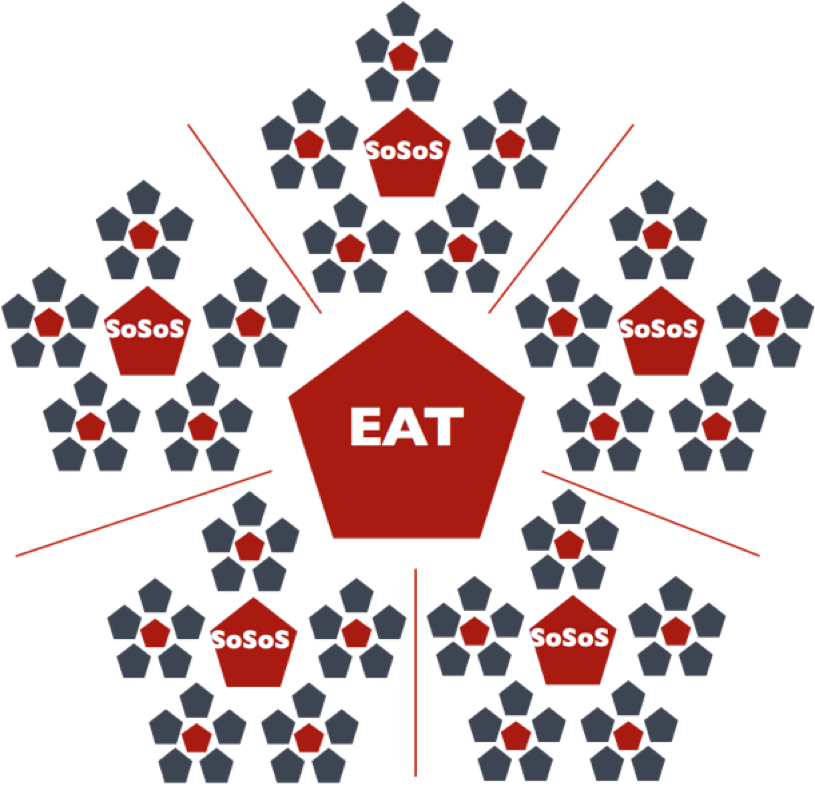
\includegraphics[width=\textwidth,height=\textheight,keepaspectratio]{SoS-EAT.png}

\subsection{EAT Backlog \& Aufgaben}
Scrum ist ein agiles Betriebssystem, das sich von traditionellem Projektmanagement
unterscheidet. Die gesamte Scrum Master Organisation berichtet an das EAT, das
dafür verantwortlich ist, dieses agile Betriebssystem in der Organisation zu
etablieren, aufrecht zu erhalten und die Implementierung in der Organisation zu
verbessern.
Die Rolle des EAT besteht darin, ein Organisations-Transformations Backlog zu
erstellen – eine priorisierte Liste aller agilen Initiativen, die umgesetzt
werden müssen - und deren Umsetzung sicherzustellen. Gibt es z.B. in der
bisherigen Organisation einen traditionellen Produktentwicklungsprozess, muss
ein neuer, agiler Produktentwicklungsprozess entwickelt, umgesetzt und
unterstützt werden. Compliance und Qualität werden dann typischerweise besser
unterstützt, müssen aber anders, mit anderen Regeln und Richtlinien, entwickelt
werden. Das EAT stellt sicher, dass eine Product Owner Organisation gegründet
und finanziert wird und dass diese Organisation im EAT vertreten ist, um
dessen Bemühungen zu unterstützen.

Das EAT ist für die Qualität von Scrum innerhalb der Organisation verantwortlich.
Es ist u.a. zuständig für:
\begin{itemize}
\item die Schaffung eines agilen Betriebssystems für ein in der Organisation
skalierbares Referenzmodell, einschließlich betrieblicher Regeln, Prozesse und
Richtlinien, um Agilität zu ermöglichen.
\item Messung und Verbesserung der Qualität von Scrum in der Organisation.
\item den Aufbau von Kompetenzen innerhalb der Organisation, um Business Agility zu ermöglichen.
\item den Aufbau eines Centers für kontinuierliches Lernen für Scrum Professionals.
\item das Ausprobieren neuer Arbeitsweisen zu unterstützen.
\end{itemize}
Schließlich muss das EAT eine korrespondierende Product Owner Organisation
aufbauen und unterstützen. Sie besteht aus verbundenen Product Ownern, die die
SoS spiegeln und ihre PO Funktionen skalieren.

\subsection{Outputs/Outcomes des Scrum Master Zyklus}
Die Scrum Master Organisation (SoS, SoSoS, EAT) arbeitet als Ganzes, um die
übrigen Komponenten des Scrum Master Zyklus auszuführen: \textbf{Kontinuierliche Verbesserung
und Hindernisbeseitigung, Cross-Team Koordination und Auslieferung}.

Die Ziele von Kontinuierlicher Verbesserung und Hindernisbeseitigung sind:
\begin{itemize}
\item Hindernisse zu identifizieren und sie als Chancen zu deuten.
\item Eine gesunde und strukturierte Umgebung aufrecht zu erhalten, in der
Hindernisse priorisiert und beseitigt werden und Verbesserungen überprüft
und verifiziert werden.
\item Sichtbarkeit in der Organisation sicherzustellen, um Veränderungen zu bewirken.
\end{itemize}
Die Ziele von Cross-Team Koordination sind:
\begin{itemize}
\item ähnliche Prozessen über mehrere zusammenhängende Teams zu koordinieren.
\item Abhängigkeiten zwischen Teams zu mildern, damit sie nicht zu Hindernissen werden.
\item die Abstimmung von Team Normen und Regeln aufrechtzuerhalten, um konsistente
Ergebnisse zu gewährleisten.
\end{itemize}

Das SoS ist ein Releaseteam, daher fällt die Auslieferung des Produktes unter
seine Verantwortung, während die Product Owner über die Inhalte des Releases
entscheiden. Die Ziele der Komponente Auslieferung sind daher:

\begin{itemize}
\item Auslieferung eines konsistenten Flusses von wertvollen, fertiggestellten Produkten an Kunden.
\item Integration der Arbeitsergebnisse verschiedener Teams zu einem nahtlosen Produkt.
\item qualitativ hochwertige Customer Experience sicherzustellen.
\end{itemize}

\section{Der Product Owner Zyklus}
\subsection{Das ``Was'' koordinieren – Das Product Owner Team}
Eine Gruppe von Product Ownern, die ein gemeinsames Backlog für ein Netzwerk
von Teams koordinieren müssen, sind selbst ein Team, das \textbf{Product Owner Team}
genannt wird. Für jedes SoS gibt es ein zugehöriges Product Owner Team, das die
Prioritäten der Teams entlang eines gemeinsamen Pfades ausrichtet. So können die
Backlogs ihrer Teams koordiniert, mit den Stakeholdern abgestimmt und von
ihnen unterstützt werden.

Der Product Owner eines Teams ist verantwortlich für die Erstellung und
Priorisierung des Team Backlogs und kann Backlog Einträge aus dem gemeinsamen
MetaScrum Backlog in das Team Backlog ziehen oder nach eigenem Ermessen
unabhängige Backlog Einträge erstellen.

Product Owner Teams halten eine skalierte Version des Backlog Refinement ab, das \textbf{MetaScrum}:
\begin{itemize}
\item Jeder Team PO (oder sein/ihr Vertreter) muss am MetaScrum teilnehmen, in dem Stakeholder das Backlog des Product Owner Teams begutachten und Strategie-, Ressourcen- und Zeitthemen adressieren.
\item Dieses Event ist Forum für Führung, Stakeholder oder weitere
Kunden, um ihre Präferenzen auszudrücken
\end{itemize}
Dieses Event findet so oft wie nötig statt, jedoch mindestens einmal pro Sprint,
um ein Ready Backlog auf Product Owner Team Ebene sicherzustellen.

Die wesentlichen Funktionen des Product Owner Teams sind:
\begin{itemize}
\item eine übergreifende Produktvision zu gestalten \& sie in der Organisation sichtbar zu machen.
\item Einverständnis mit den wesentlichen Stakeholdern zu schaffen, um die
Unterstützung für die Verwirklichung des Backlogs sicherzustellen
\item Erstellung eines einheitlichen, priorisierten Backlogs; sicherstellen, dass
Doppelarbeiten ausgeschlossen sind
\item Sicherstellen, dass Hindernisse und Themen zu technischen Schulden im Backlog richtig priorisiert werden.
\item Festlegung einer minimalen einheitlichen ``Definition of Done'', die für alle Teams im SoS gilt
\item Beseitigung von Abhängigkeiten, die von den Teams gemeldet werden.
\item Erstellung einer koordinierten Roadmap und eines koordinierten Releaseplanes.
\item Entscheidung für und Beobachtung von Metriken, die Erkenntnisse über das Produkt und den Markt liefern.
\end{itemize}
Product Owner Teams funktionieren, genauso wie SoSs, wie Scrum Teams. Als solche
benötigen sie einen Scrum Master, der das Team während Diskussionen fokussiert
hält. Außerdem benötigen sie eine einzelne Person, die dafür verantwortlich ist,
die Erstellung eines einzelnen Product Backlogs für alle Teams im Scrum of Scrums
zu koordinieren. Diese Person wird bezeichnet als \textbf{Chief Product Owner}.

\subsection{Der Chief Product Owner (CPO)}
Die Chief Product Owner koordinieren die Prioritäten unter den Product Ownern,
die mit einzelnen Teams arbeiten. Sie richten Backlog Prioritäten entlang der
Bedürfnisse der Stakeholder und Kunden aus. Genau wie ein SoSM kann der CPO ein
PO eines individuellen Teams sein, der sich dazu entschließt, diese Rolle
ebenfalls auszufüllen, oder es kann eine Person sein, die besonders dafür
benannt wurde. Die wesentlichen Aufgaben sind dieselben, wie die eines
regulären PO, nur skaliert:
\begin{itemize}
\item Eine Strategische Vision für das gesamte Produkt zu bestimmen.
\item Ein einziges, priorisiertes Backlog zu erstellen, dessen Wert von
allen Teams geliefert wird
\begin{itemize}
\item diese Einträge wären größere Product Backlog Einträge als die eines Team PO.
\end{itemize}
\item Eng mit dem zugehörigen SoSM zusammenzuarbeiten, so dass der Releaseplan, den das Product Owner Team generiert, effizient umgesetzt werden kann.
\item Kundenfeedback zum Produkt aufzunehmen und das Backlog entsprechend anzupassen.
\item Das MetaScrum zu leiten, in dem das Product Backlog gezeigt und die Abstimmung mit Stakeholdern erzielt wird.
\end{itemize}

\subsection{Das Product Owner Team skalieren}
Genau wie sich SoSs zu einem SoSoS ausdehnen können, können Product Owner
Teams durch denselben Mechanismus erweitert werden. Es gibt weder einen
besonderen Begriff für diese erweiterten Einheiten, noch haben deren CPOs
besondere, erweiterte Titel. Wir ermutigen jede Organisation, ihre eigenen zu
entwickeln. Für die folgenden Diagramme haben wir mit jeder jeweils höheren
Skalierungsebene den Titel des Product Owners um ein zusätzliches ``Chief''
ergänzt.

Die Product Owner Teams treffen sich regelmäßig (mindestens einmal pro Sprint) mit wesentlichen Stakeholdern, um das Backlog für die gesamte Organisation auszurichten. Dieses Treffen heißt MetaScrum und wird vom Chief Product Owner geleitet. Hier können Prioritäten verhandelt, Budgets verändert und Teams neu ausgerichtet werden, um den Wert zu maximieren, der an den Markt ausgeliefert wird.

%\pagebreak
Einige Beispieldiagramme::

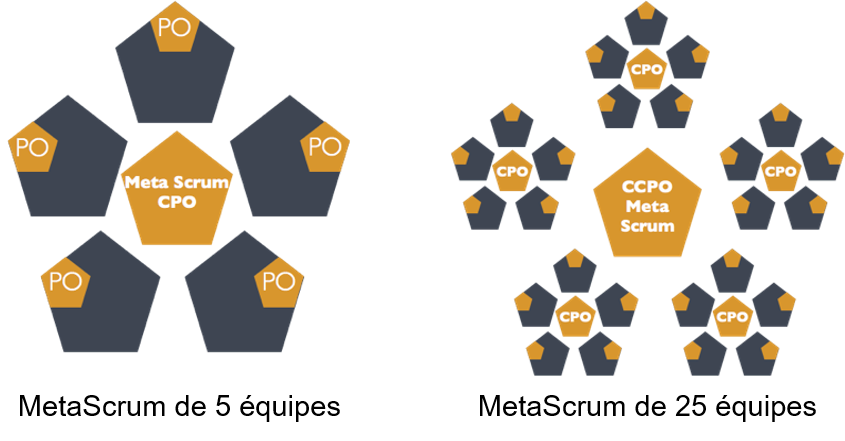
\includegraphics[width=1.0\linewidth]{MetaScrum-R2.png}

\textbf{ANMERKUNG:} Wie oben erwähnt, repräsentieren diese Fünfecke Scrum Teams
und Product Owner Teams mit der idealen Größe. Diese Diagramme sollen nur als
Beispiele dienen, Ihr eigenes Organisationsdiagramm kann stark hiervon abweichen.


\subsection{Das Executive MetaScrum (EMS)}
Die Product Owner Teams ermöglichen ein Netzwerk Design von Product Ownern, das
gemeinsam mit den dazugehörigen SoSs unendlich skaliert werden kann. Das
Product Owner Team für die gesamte agile Organisation trifft sich mit
wesentlichen Stakeholdern zum \textbf{Executive MetaScrum}. Dem EMS gehört
die unternehmerische Vision und es bestimmt die strategischen Prioritäten.
Das EMS richtet alle Teams an gemeinsamen Zielen aus.

Beispieldiagramm eines EMS, das 5 Gruppen von 25 Teams koordiniert:

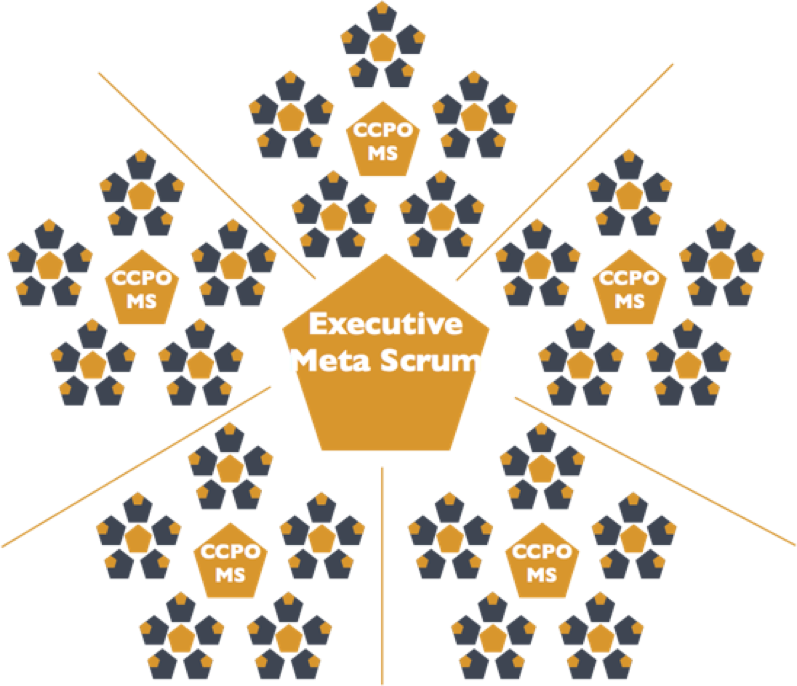
\includegraphics[width=1.0\linewidth]{ExecMetaScrum.png}

\subsection{Outputs/Outcomes der Product Owner Organisation}
Die PO Organisation (die Product Owner, die CPOs und das Executive MetaScrum)
arbeitet als Ganzes, um die Komponenten des Product Owner Zyklus zu bedienen:
\textbf{Strategische Vision, Backlog Priorisierung, Backlog Decomposition \& Refinement und Release Planung}.

Die Ziele bei der Bestimmung einer Strategischen Vision sind:
\begin{itemize}
\item die gesamte Organisation eindeutig entlang eines gemeinsamen Pfades vorwärts auszurichten.
\item überzeugend zu formulieren, warum die Organisation existiert.
\item zu beschreiben, wie die Organisation wesentliche Faktoren nutzt, um ihre Mission zu unterstützen.
\item sich ständig anzupassen, um auf sich schnell ändernde Marktbedingungen reagieren zu können.
\end{itemize}
Die Ziele der Backlog Priorisierung sind:
\begin{itemize}
\item eine klare Reihenfolge zu identifizieren für Produkte, Features und
Services, die geliefert werden sollen
\item die Wertschöpfung, die Risikominderung und interne Abhängigkeiten bei der
Priorisierung des Backlogs zu berücksichtigen.
\item übergeordnete Initiativen für die gesamte Organisation noch vor Backlog Decomposition & Refinement zu priorisieren.
\end{itemize}
Die Ziele von Backlog Decomposition \& Refinement sind:
\begin{itemize}
\item komplexe Projekte und Produkte in funktional unabhängige Elemente
herunterzubrechen, die von einem Team innerhalb eines Sprints fertiggestellt
werden können
\item Emergente Anforderungen und Kundenfeedback zu sammeln und auszuwerten.
\item Sicherzustellen, dass alle Backlogeinträge tatsächlich ``ready'' sind,
sodass sie von den Teams in den Sprint gezogen werden können.
\end{itemize}
Die Ziele der Release Planung sind:
\begin{itemize}
\item die Lieferung von Kernfeatures und Leistungsfähigkeiten vorherzusagen.
\item Lieferungserwartungen gegenüber Stakeholdern zu kommunizieren.
\item die Priorisierung nach Bedarf zu aktualisieren.
\end{itemize}

\section{Die PO/SM Zyklen verbinden}

\subsection{Feedback verstehen}
Die Komponente \textbf{Feedback} ist der zweite Punkt, an dem sich der PO-Zyklus
und der SM-Zyklus berühren. Während Feedback zum Produkt kontinuierliche
Verbesserung vorantreibt, indem es das Product Backlog anpasst, treibt Feedback
zum Release kontinuierliche Verbesserung voran, indem es Auslieferungsmechanismen
anpasst. Die Ziele bei der Gewinnung und Analyse von Feedback sind:
\begin{itemize}
\item unsere Annahmen zu validieren.
\item zu verstehen, wie Kunden das Produkt benutzen und mit ihm interagieren.
\item Ideen für neue Features und Funktionalitäten zu erfassen.
\item Verbesserungen zu bestehender Funktionalität zu definieren.
\item den Fortschritt hinsichtlich Projekt- / Produktfertigstellung zu aktualisieren, um die Releaseplanung und Abstimmung mit den Stakeholdern zu verbessern.
\item Verbesserungen für Auslieferungsmethoden und -mechanismen zu identifizieren.
\end{itemize}

\subsection{Metriken \& Transparenz}
Radikale Transparenz essenziell, damit Scrum optimal funktioniert. Das ist aber
nur in einer Organisation möglich, die die Scrum Werte beherzigt. Radikale
Transparenz gibt der Organisation die Möglichkeit, ihre Fortschritte reell zu
beurteilen und die Produkte und Prozesse zu überprüfen und anzupassen. Dies ist
die Grundlage der empirischen Natur von Scrum, wie sie im Scrum Guide erklärt ist.

SM- \& PO-Zyklus benötigen Metriken, die von den jeweiligen SM- und
PO-Organisationen festgelegt werden. Metriken können sowohl für beide jeweiligen
Organisationen, als auch für einzelne Funktionen innerhalb dieser Organisationen
unterschiedlich sein. Scrum@Scale setzt kein spezifisches Set an Metriken voraus.
Aber es legt nahe, dass die Organisation mindestens:
\begin{itemize}
\item Produktivität – z. B. Veränderung der Menge an verwendbaren Arbeitsergebnissen,
die pro Sprint geliefert werden
\item Wertauslieferung – z. B. Geschäftswert pro Einheit des Teamaufwandes
\item Qualität – z. B. Fehlerrate oder Serviceausfallzeiten
\item Nachhaltigkeit – z. B. Teamzufriedenheit
\end{itemize}
misst.
Die Ziele von Metriken und Transparenz sind:
\begin{itemize}
\item alle Entscheider, inklusive der Teammitglieder, mit ausreichend Kontext zu
versorgen, um gute Entscheidungen treffen zu können.
\item Feedbackzyklen so weit wie möglich zu verkürzen um Überkorrektur zu vermeiden.
\item rminimalen zusätzlichen Aufwand durch Teams, Stakeholder und Führung zu
benötigen.
\end{itemize}

\subsection{Einige Anmerkungen zu Organisationsdesign}
Die „skalierungsfreie“ Natur von Scrum@Scale erlaubt eine Organisationsstruktur,
die komponentenbasiert ist, genau wie das Rahmenwerk selbst. Dies erlaubt
Neugewichtungen oder Umgestaltungen von Teams als Antwort auf den Markt.
Wenn eine Organisation wächst, kann es sehr wichtig sein, die Vorteile verteilter
Teams zu nutzen. Einige Unternehmen gewinnen Talente, die anderweitig nicht
verfügbar sind und sind in der Lage durch outgesourcte Entwicklung nach Bedarf
zu wachsen zu schrumpfen. Scrum@Scale zeigt, wie das ohne lange
Verzögerungszeiten, eingeschränkte Kommunikation und mindere Qualität gelingen
kann und ermöglicht lineare Skalierbarkeit sowohl in Größe als auch in globaler
Verteilung. \footnote{Sutherland, Jeff and Schoonheim,
Guido and Rustenburg, Eelco and Rijk, Maurits, ``Fully distributed scrum:
The secret sauce for hyperproductive offshored development teams'',
AGILE'08. Conference, IEEE: 339-344, 2008}

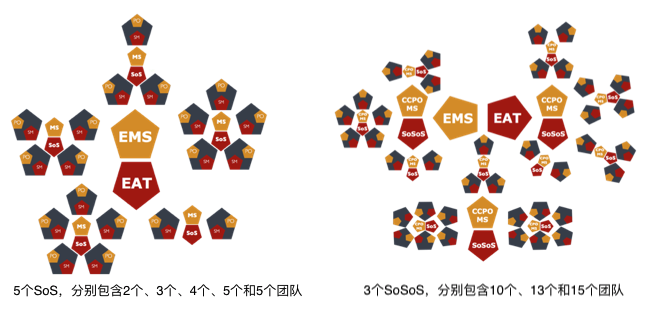
\includegraphics[width=1.0\linewidth]{VariableSoS-R2.png}
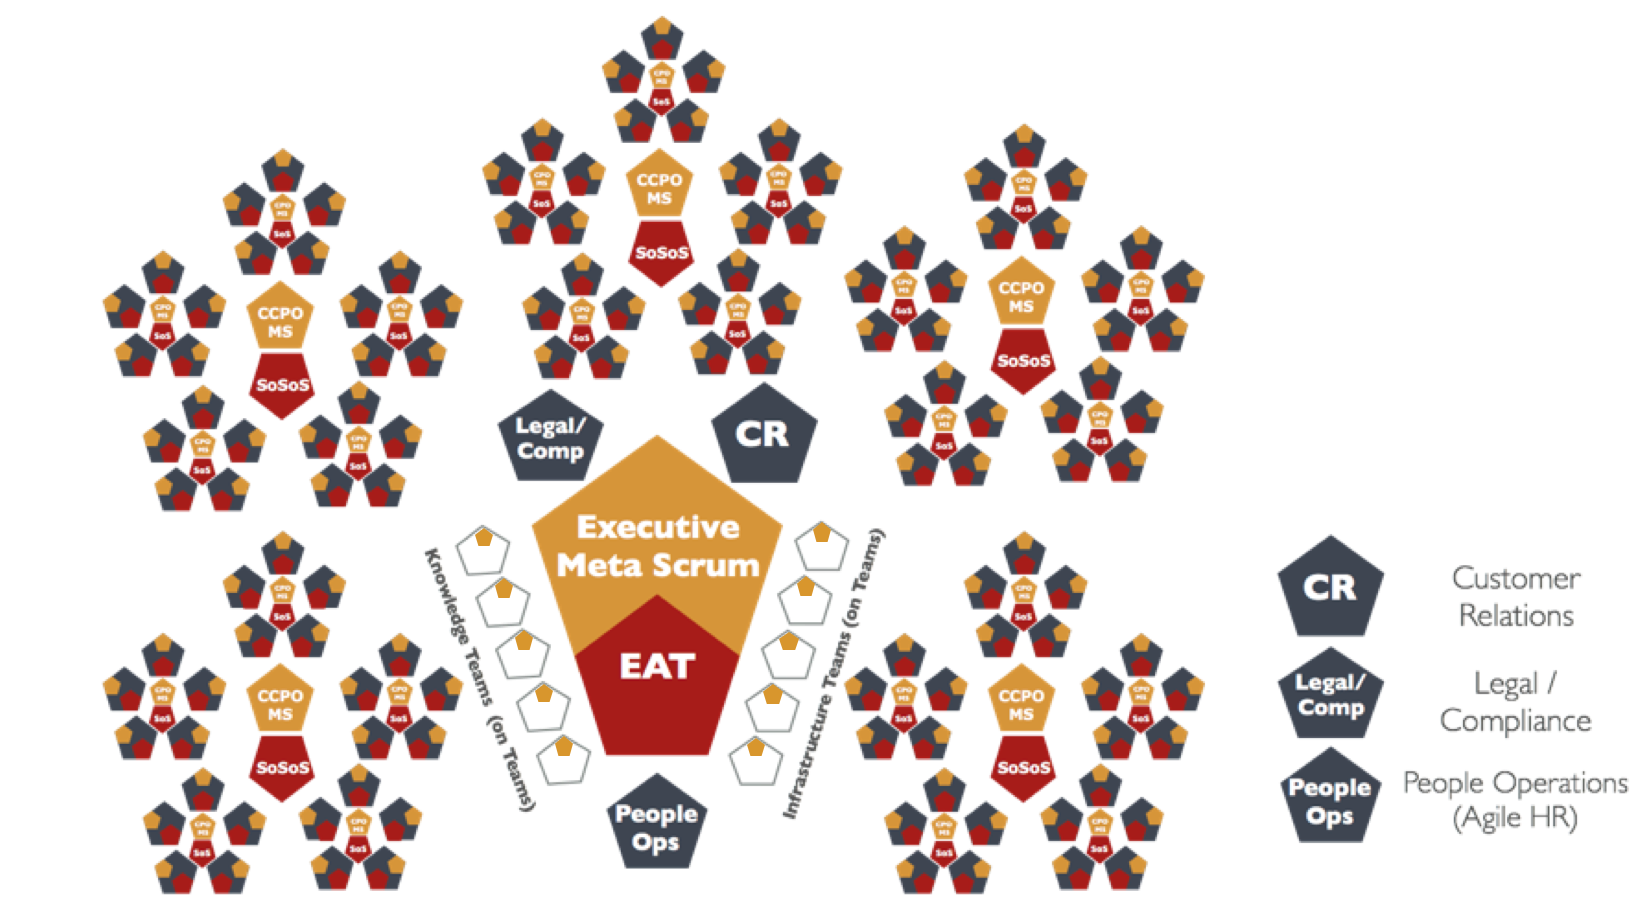
\includegraphics[width=1.0\linewidth]{OrganizationalDiagram.png}

In diesem Organisationsdiagramm sind die \textbf{Wissens- und Infrastrukturteams}
als virtuelle Spezialistenteams dargestellt. Von diesen Spezialisten gibt es zu
wenige für jedes einzelne Team. Sie koordinieren sich als Gruppe mit den Scrum
Teams über Service-Level Agreements. Ein PO nimmt die Anfragen entgegen und
erstellt daraus für jedes Spezialgebiet ein transparentes, priorisiertes Backlog.
Wichtiger Hinweis: Diese Teams sind NICHT Silos von Individuen, die
zusammensitzen (deswegen sind sie in diesem Diagramm als leere Fünfecke
dargestellt); ihre Teammitglieder sitzen in den eigentlichen Scrum Teams.
Sie bilden aber dieses eigene virtuelle Scrum zwecks Backlogverteilung und
Prozessverbesserung.

\textbf{Customer Relations, Rechtsabteilung & Compliance und People Operations}
sind hier ebenfalls als notwendige Teile der Organisation inbegriffen. Sie
existieren als eigene, unabhängige Scrum Teams, von denen alle anderen abhängen
können.

Eine letzte Anmerkung zur Darstellung des EAT \& EMS: In diesem Diagramm werden
sie als sich überschneidend dargestellt, da einige ihrer Mitglieder beiden
Teams angehören. In sehr kleinen Organisationen oder Implementierungen können
EAT \& EMS vollständig aus denselben Teammitgliedern bestehen.

\section{Schlussbemerkung}
Scrum@Scale wurde dafür entwickelt, um Produktivität zu skalieren, sodass die
gesamte Organisation den doppelten Wert in der Hälfte der Zeit schafft, mit
besserer Qualität und signifikant besseren Arbeitsbedingungen. Große
Organisationen, die dieses Rahmenwerk richtig implementieren, können die Kosten
für ihre Produkte und Services senken und gleichzeitig Qualität verbessern und
Innovation vorantreiben.

Scrum@Scale ist dafür entwickelt, eine Organisation mit Scrum zu sättigen. Alle Teams
einschließlich Führung, HR, Rechtsabteilung, Beratung \& Training und Produkt-
und Serviceteams wenden Scrum in gleichem Stil an und straffen und verbessern damit die Organisation.

Gut implementiertes Scrum kann eine gesamte Organisation steuern.

\section{Danksagungen}
Wir bedanken uns bei IDX für die Einrichtung der Scrum of Scrums, die zum ersten
Mal eine Skalierung von hunderten Teams ermöglichten,\footnote{Sutherland, Jeff,
``Inventing and Reinventing SCRUM in five Companies'', Sur le site officiel
de l'alliance agile, 2001} PatientKeeper für die Einrichtung des
MetaScrum,\footnote{Sutherland, Jeff, ``Future of scrum: Parallel pipelining of
sprints in complex projects'', Proceedings of the Agile Development Conference,
IEEE Computer Society 90-102,  2005.} das schnelle Auslieferung von innovativen
Produkten ermöglichte, und OpenView Venture Partners dafür, dass sie Scrum über
die gesamte Organisation skaliert haben.\footnote{Sutherland, Jeff and Altman,
Igor, ``Take no prisoners: How a venture capital group does scrum'', Agile
Conference, 2009. AGILE'09, IEEE 350-355.  2009} Wir schätzen den Input von Intel
mit über 25000 Menschen, die Scrum anwenden und uns gelehrt haben, dass
``nichts skaliert'', außer einer skalierungsfreien Architektur und SAP mit der
größten Scrum Team Produktorganisation, die uns gelehrt hat, dass die
Beteiligung von Management im MetaScrum essenziell ist, um 2000 Scrum Teams
zusammen arbeiten zu lassen.


Die agilen Coaches und Trainer, die diese Konzepte bei Amazon, GE, 3M, Toyota,
Spotify, Maersk, Comcast, AT&T implementiert haben, und viele andere Unternehmen,
die mit Jeff Sutherland zusammengearbeitet haben, waren hilfreich dabei, diese
Konzepte in zahlreichen Unternehmen in verschiedenen Domänen zu testen.

Zuletzt waren Avi Schneier und Alex Sutherland unersetzlich bei der Formulierung
und Überarbeitung dieses Dokuments.

\pagebreak

\printbibliography

\section{Übersetzung}
Diesen Guide haben Alisa Stolze und Peter Fischbach im Januar 2018 übersetzt.
Letzte Bearbeitung am 20.01.2019. 
\end{document}
